\chapter{Statistical results and interpretation}
\section{Likelihood model}
\label{sec:likelihood}

Consider a given category of event as defined by \njet, \nb~and \scalht, which are in the following identified with \htcat. 
In each category, the signal is extracted using the discriminating variable \mht. 
Templates of the \mht~distribution are built for the signal and the background processes 
using the simulated samples described in Sec.?? The \mht binning is tabulated in Sec.~\ref{sec:mhtBinning}.
The binning of the templates is chosen taking into account both the limited statistics in the simulation and 
the control of the background in data. 
A maximum statistical uncertainty from the simulated events of 50\% (corresponding to four unweighted events) 
is required in each bin of the template in order to ensure a statistically meaningful prediction. 
A minimum bin width constraint of 50 GeV is applied in order to reduce the bin-by-bin migration 
due to the finite \mht resolution.

The likelihood model in each bin in \mht~and \htcat~is split into hadronic and control components linked
by floating parameters for the prediction. In one \htcat~category, j, the hadronic component may be written as,

\begin{multline}
\label{eq:hadronicLikelihood}
\mathcal{L}^{j}_{\mathrm{had}} = \prod_i \mathrm{Pois}(n^{j,i}_{\mathrm{had}} |\, b^{j,i}_{\zInv~,had}\times\phi^{j}(\mu\rightarrow\zInv~)\times a^{j}\times\rho^{j,i}_{\zInv~,had}\, + \\ 
b^{j,i}_{\ttW,\mathrm{had}}\times\phi^{j}(\mu\rightarrow\ttW)\times a^{j}\times\rho^{j,i}_{\ttW,had}\, + b^{j,i}_{\text{QCD},had}\times\omega^{j,i}_{\text{QCD},had}\\\
+ \,r\times s^{j,i}_{\mathrm{had}}\times\rho^{j,i}_{s,had}) 
\end{multline}

where $b^{j}$ are the predicted number of events from simulation for the electroweak
backgrounds and from the method described in~\ref{sec:qcd-pred} for the QCD multijet component ($b^{j,i}_{\text{QCD},had}$), 
the $a^{j}$ parameter is unconstrained and fully correlated with the prediction of the signal region may be connected 
to the control region (see below), while the $\phi^{j,i}$ contain the systematic uncertainties on the 
transfer factors on the relevant prediction from the data driven tests described in Section ?? and the 
$\rho^{j}$ contain the systematics from variations in simulation as well as the uncertainty from the limited number of 
simulated events for background and signal (described in Section ?? and ??), r is an uncontrained parameter 
termed the \emph{signal strength}, and $\omega_{\text{QCD}}$ contains the uncertainties on the QCD multijet component. 
The constraint terms for the systematic uncertainties are detailed in Section ??.

The component of the likelihood for the \mj~control region, which is not categorised in \mht, can be written as

\begin{equation}
\label{eq:muLikelihood}
\mathcal{L}^{j}_{\mathrm{\mu}} = \mathrm{Pois}(n^{j}_{\mathrm{\mu}} |\, b^{j}_{\mu}\times a^{j}\times\rho^{j}_{\mu} + \,r \times s^{j}_{\mathrm{\mu}}\times\rho^{j}_{s,\mu})
\end{equation}

similarly to Equation, $\rho^{j}_{\mu}$ contains the uncertainty in the \htcat from variations in simulation. The $s^{j}_{\mathrm{\mu}}$
econdes the signal \emph{contamination} in the control region which is small by design. The connection between the control and signal region
is encoded by the unconstrained $a^{j}$ parameter. The \zInv~component in the signal 
region is also predicted using the \gj and \mmj regions. By rewriting $\phi^{j}(\mu\rightarrow\zInv~)\times a^{j}$ and $\phi^{j}(\mu\rightarrow\ttW)\times a^{j}$
as ${a'}(\mu\rightarrow\zInv~)$ and $a'(\mu\rightarrow\ttW~)$ respectively, the connections to the \gj~and \mmj~regions
may be written as, 

\begin{align}
\label{eq:mumuLikelihood}
\mathcal{L}^{j}_{\mathrm{\mu\mu}} &= \mathrm{Pois}(n^{j}_{\mathrm{\mu\mu}} |\, b^{j}_{\mu\mu}\times 
\left({a'}^{j}/\phi^{j}(\mu\mu\rightarrow\zInv~)\right)\times\rho^{j}_{\mu\mu} + \,r\times s^{j}_{\mathrm{\mu\mu}}\times\rho^{j}_{s,\mu\mu}) \\
\mathcal{L}^{j}_{\mathrm{\gamma}} &= \mathrm{Pois}(n^{j}_{\mathrm{\gamma}} |\, b^{j}_{\gamma}\times 
\left({a'}^{j}/\phi^{j}(\gamma\rightarrow\zInv~)\right)\times\rho^{j}_{\gamma} + \,r\times s^{j}_{\mathrm{\gamma}}\times\rho^{j}_{s,\gamma})
\end{align}

where parameters are defined as in Equations~\ref{eq:hadronicLikelihood} and~\ref{eq:muLikelihood}. 
The $\phi^{j}$ appear on the denominator as the connection between the control and signal region is 
inverted.

The modifier and constraint terms of the parameters representing the systematic uncertainties and 
connections between control and signal regions, \emph{nuisance parameters}, can be summarised as,
\begin{itemize}
\item The transfer factor systematics (in $\phi$) and uncertinaties on the QCD multijet contribution (in $\omega$)  
are taken to be \emph{log normal} uncertainties such that the logarithm of the variable has 
a Gaussian (normal) constraint~\cite{templateMorphing}. These uncertainties are correlated per topology and \scalht bin 
(pair of \scalht bin for uncertainties derived using \mmj)
\item The systematic uncertainties from variations in simulation (in $\rho$) are included using vertical template morphing.
The yields are interpolated quadratically between the $\pm 1\sigma$ variations for each source of
uncertainty and extrapolated linearly beyond this range~\cite{templateMorphing}. The constraint term is Gaussian
with mean 0 and width 1. These uncertainties are fully correlated across all categories.
\item The poisson uncertainty due to the limited number of simulated events is approximated using
two parameters per bin which multply the total background and signal contributions and which 
are Gaussian constrained. These uncertainties are fully uncorrelated across all categories.
\end{itemize}

The total likelihood can be written as a product over all \htcat~bins,

\begin{equation}
\label{eq:totalLikelihood}
\mathcal{L} = \prod_{j\in\htcat} \mathcal{L}^{j}_{\mathrm{had}} \times \mathcal{L}^{j}_{\mathrm{\mu\mu}} 
\times \mathcal{L}^{j}_{\mathrm{\gamma}} \times \mathcal{L}^{j}_{\mathrm{\mu}}
\end{equation}


\section{Results of the fit to data}

The expected number of events from the Standard Model backgrounds are determined from 
a simultaneous fit over all parameters using data from the control regions only, \emph{CR-only fit},
as well as using data from all regions, \emph{full fit}. The CR-only fit provides the 
best representation of the background predictions of the \alphat~search from the control regions.

In Figures~\ref{fig:mono},~\ref{fig:asym} and ~\ref{fig:sym} the results of the CR-only fit and the full fit are presented in all \scalht, \njet 
and \nb~categories under a standard model only hypothesis (r = 0) for the monojet, asymmetric 
and symmetric categories respectively. No significant tension is observed between the predictions
and data. Additionally, in Figure~\ref{fig:mht-templates}, the distribution in \mht for representative 
categories of \scalht, \njet and \nb, sensitive to hadronic SUSY models with \TeV scale squarks and gluinos, 
shows good agreement between prediction and data.

The fine categorisation can complicate the comprehension of the global agreement between data and 
prediction across the signal region. In Section ??, the result is presented using 
\emph{aggregated region} in which the categorisation is simplified. 

\begin{figure}[!h]
  \begin{center}
    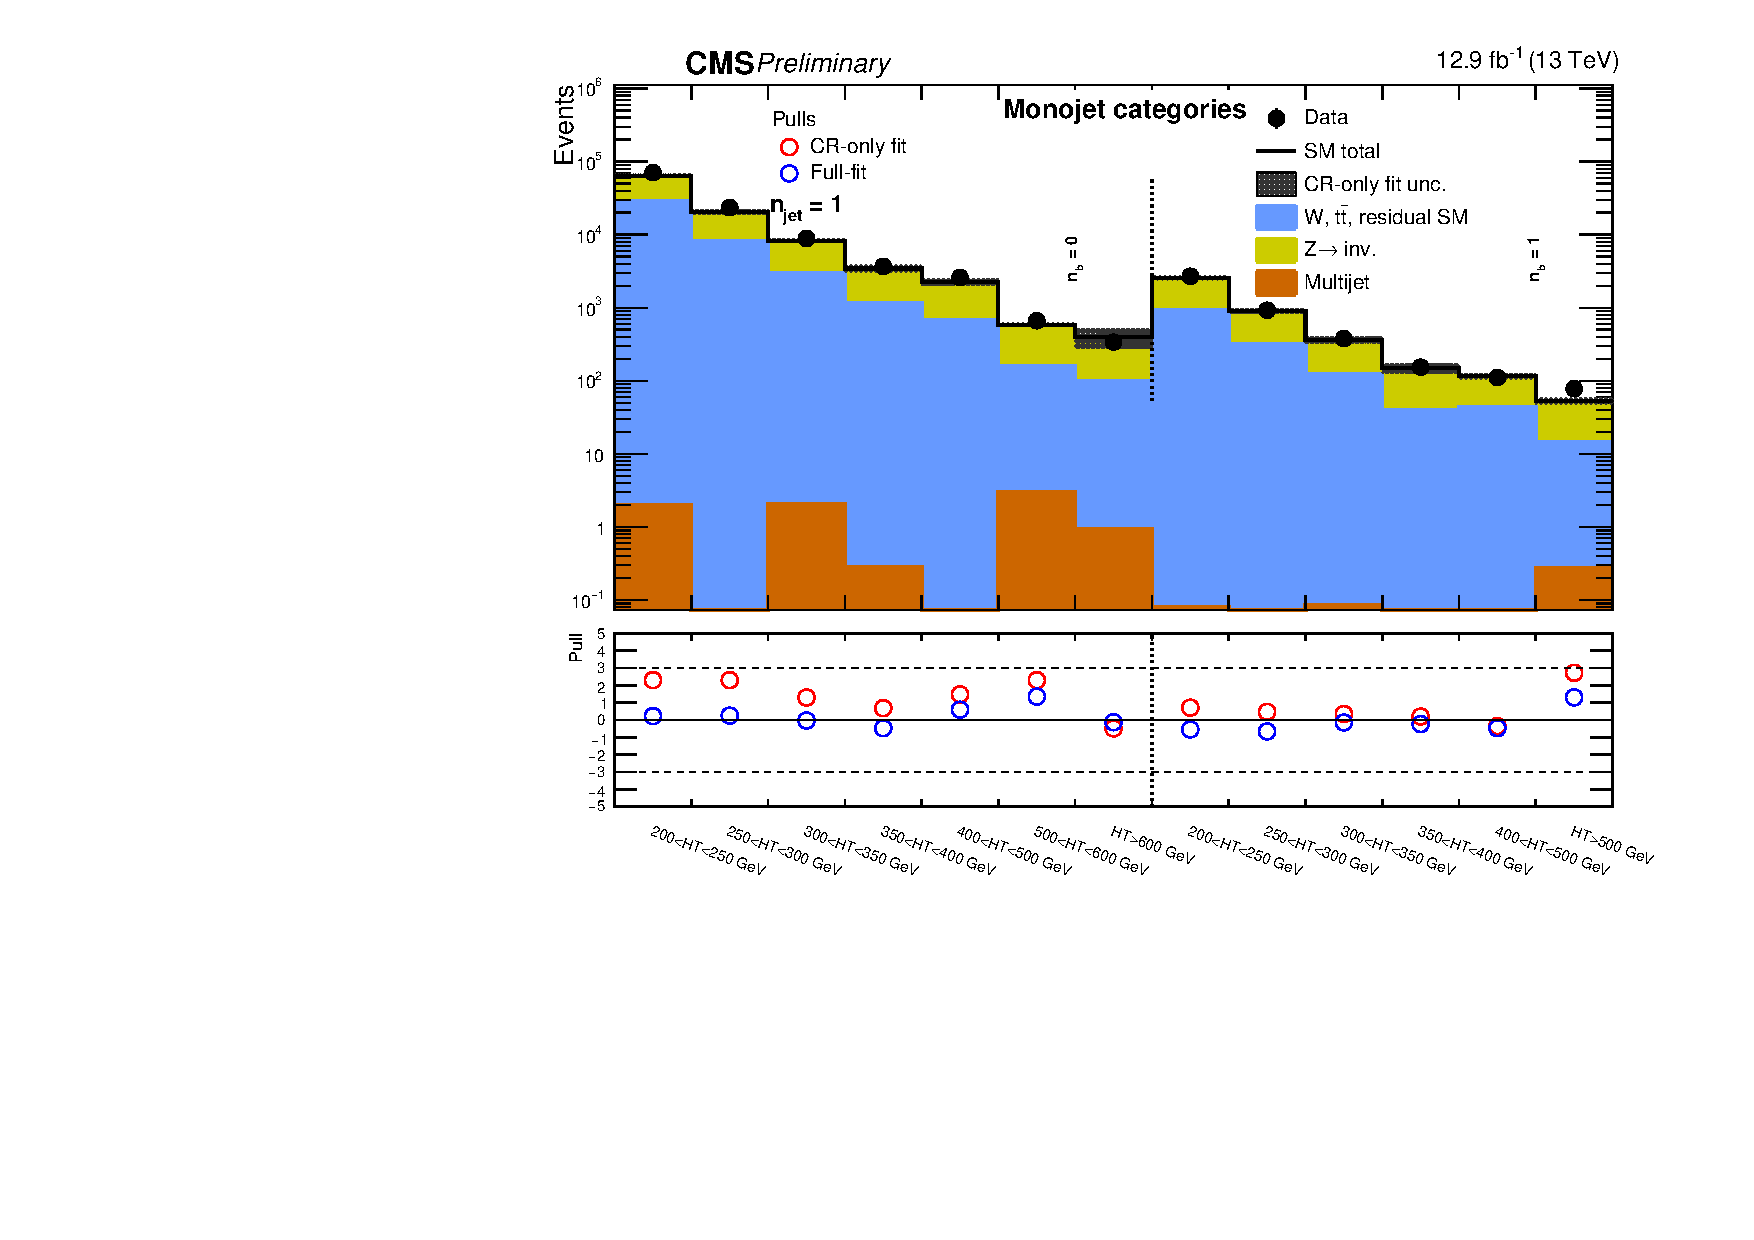
\includegraphics[width=0.7\textwidth]{Figures/statisticalResults/summaryPlot_Monojet_prefit_overlay_fit_b}
    \caption{(Top panel) Event yields observed in data (solid circles) 
	with associated Poisson uncertainty represented by error bars 
	are compared to SM predictions with associated uncertainties (black
      histogram with shaded band) from a CR-only fit as a function of
      \nb and \scalht for the monojet topology in the
      signal region. (Bottom panel). The significance of deviations
      (pulls) observed in data with respect to the SM expectations
      from the CR-only (red circles) and full fit (blue circles). The
      pulls are indicative only and cannot be considered
      independently.}
    \label{fig:mono}
  \end{center}
\end{figure}

\begin{figure}[!h]
  \begin{center}
    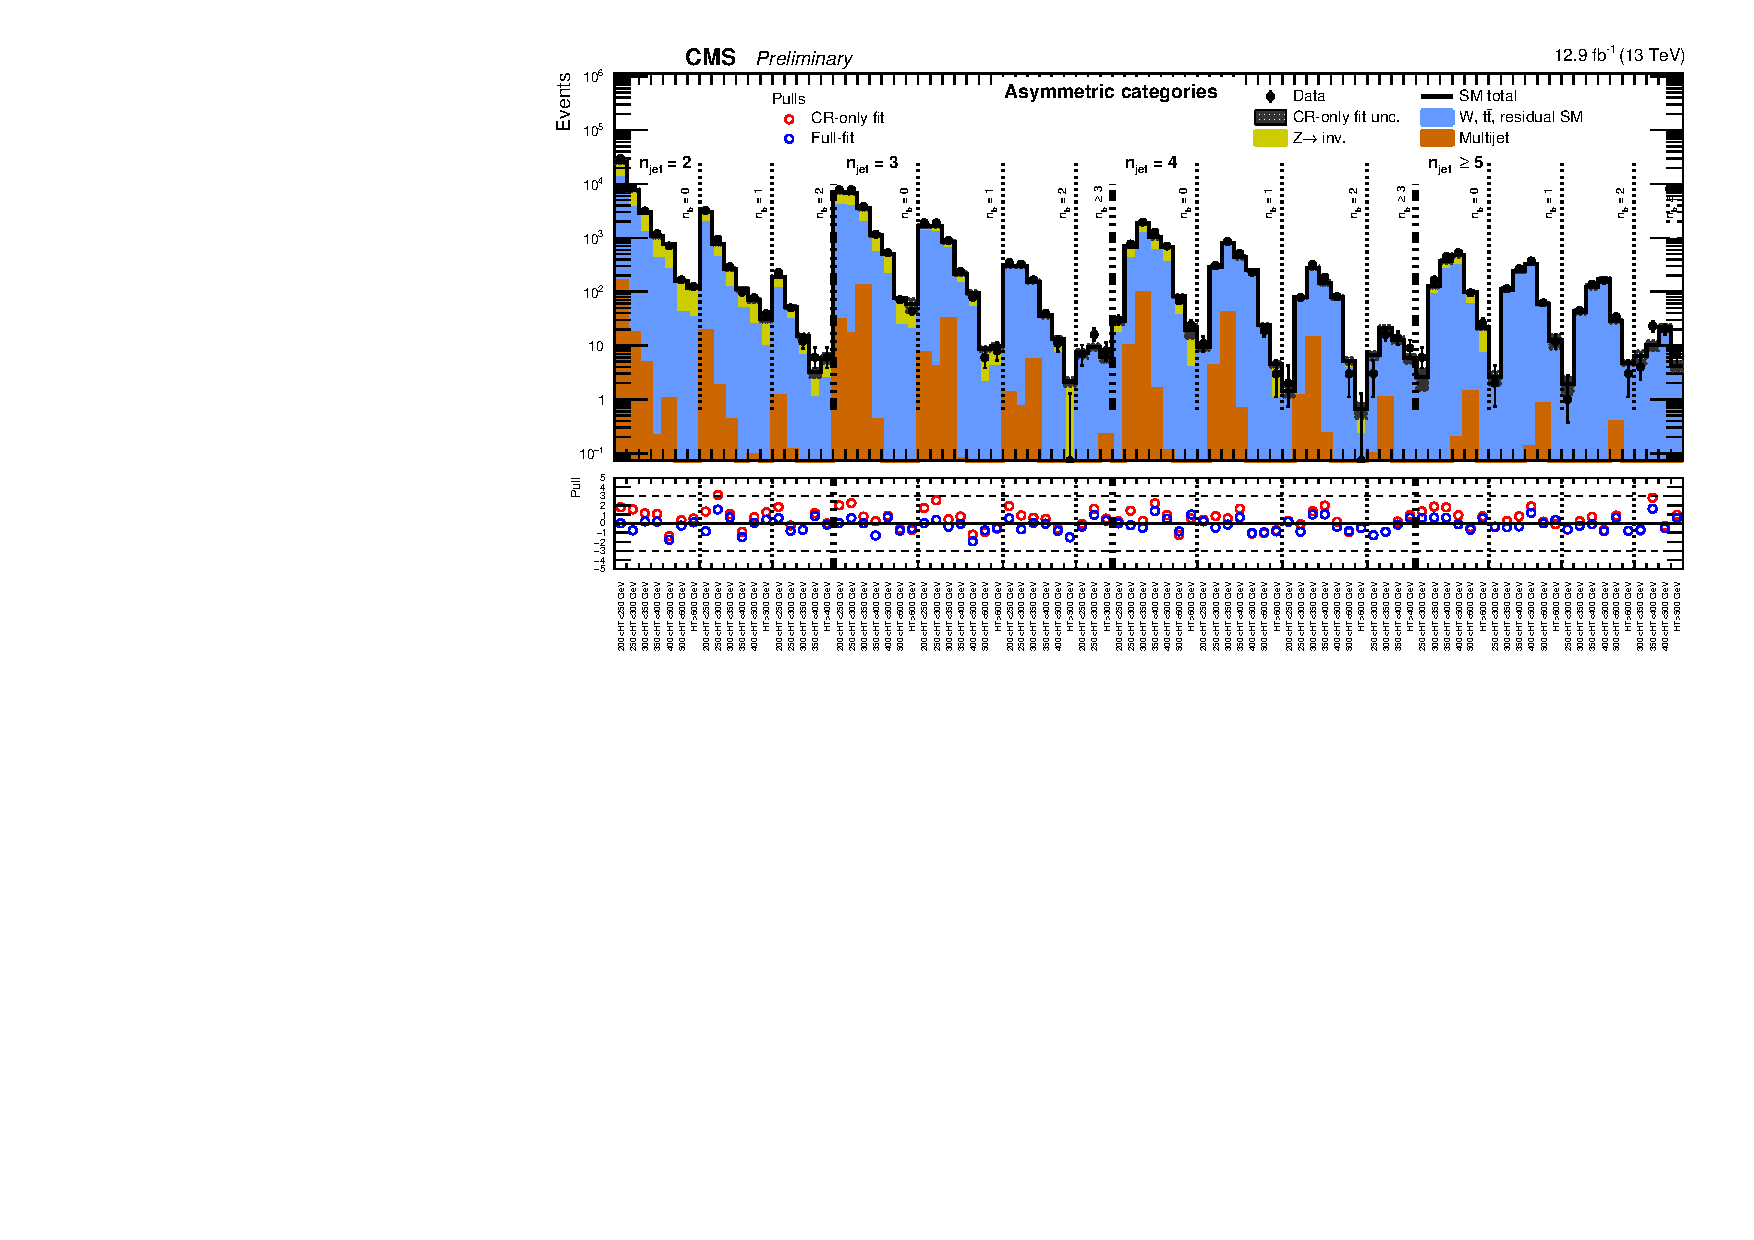
\includegraphics[angle=90,width=0.7\textwidth]{Figures/statisticalResults/summaryPlot_Asymmetric_prefit_overlay_fit_b}
    \caption{(Top panel) Event yields observed in data (solid circles) 
	with associated Poisson uncertainty represented by error bars 
	are compared to SM predictions with associated uncertainties (black
      histogram with shaded band) from a CR-only fit as a function of
      \njet, \nb and \scalht for the asymmetric topology in the
      signal region. (Bottom panel). The significance of deviations
      (pulls) observed in data with respect to the SM expectations
      from the CR-only (red circles) and full fit (blue circles). The
      pulls are indicative only and cannot be considered
      independently.}
    \label{fig:asym}
  \end{center}
\end{figure}

\begin{figure}[!h]
  \begin{center}
    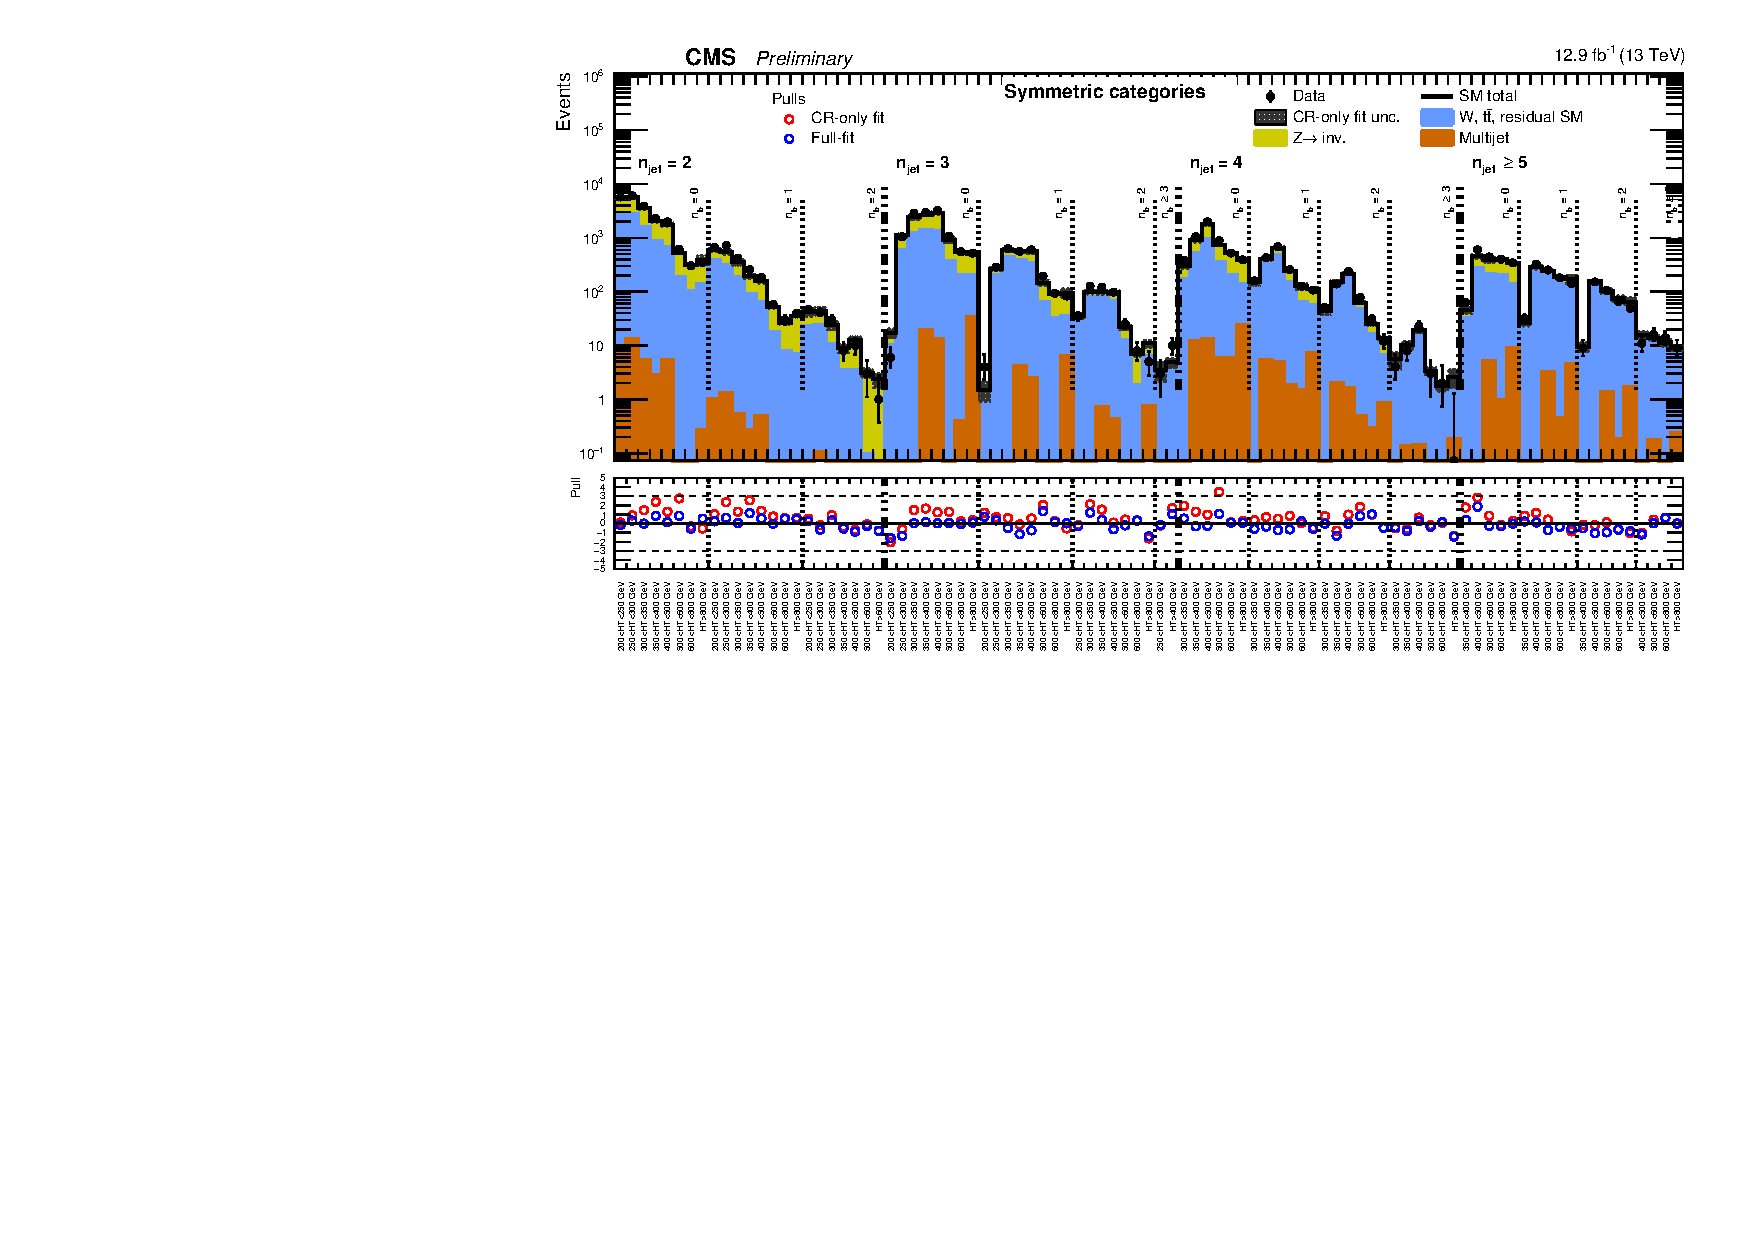
\includegraphics[angle=90,width=0.7\textwidth]{Figures/statisticalResults/summaryPlot_Symmetric_prefit_overlay_fit_b}
    \caption{(Top panel) Event yields observed in data (solid circles) 
	with associated Poisson uncertainty represented by error bars 
	are compared to SM predictions with associated uncertainties (black
      histogram with shaded band) from a CR-only fit as a function of
      \njet, \nb and \scalht for the symmetric topology in the
      signal region. (Bottom panel). The significance of deviations
      (pulls) observed in data with respect to the SM expectations
      from the CR-only (red circles) and full fit (blue circles). The
      pulls are indicative only and cannot be considered
      independently.}
    \label{fig:sym}
  \end{center}
\end{figure}

\begin{figure}[!tbhp]
  \begin{center}
    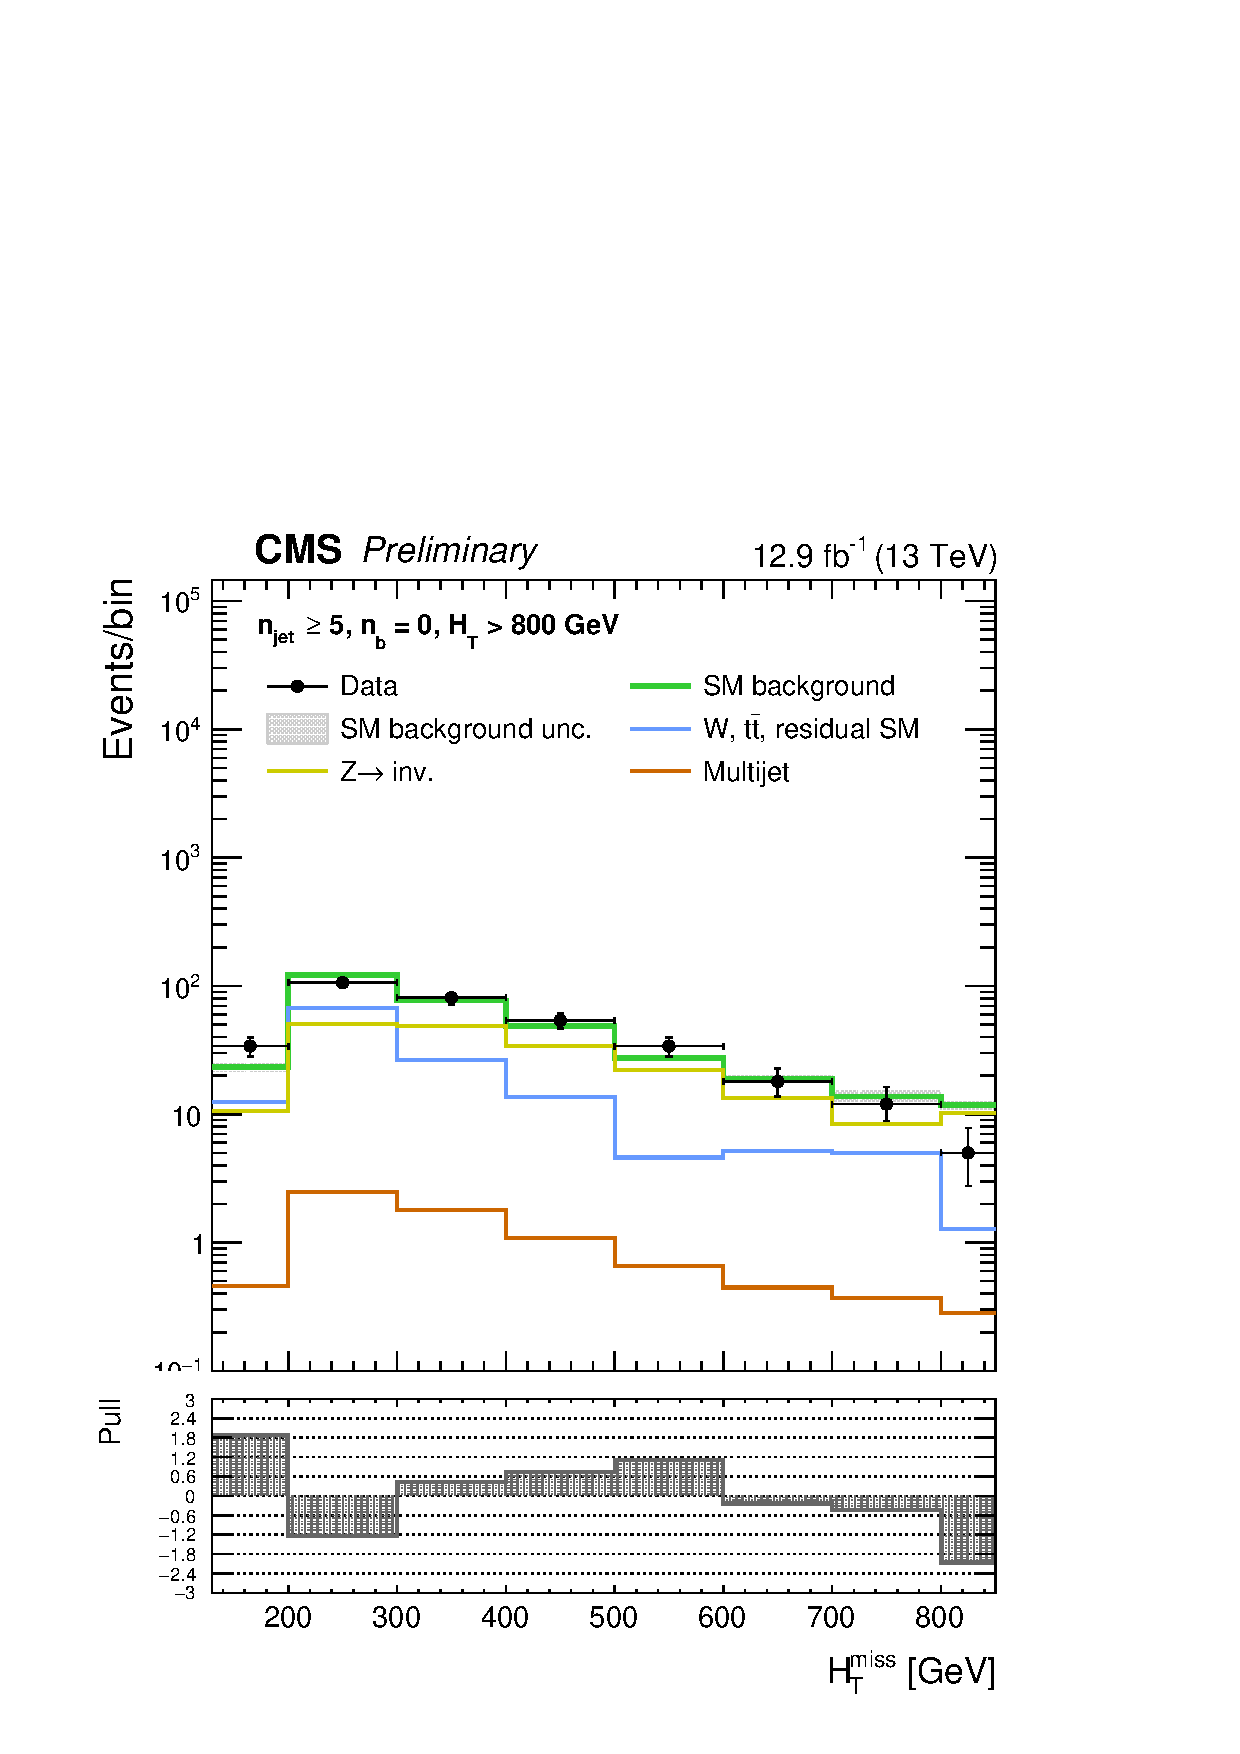
\includegraphics[width=0.49\textwidth]{Figures/statisticalResults/mhtShape_eq0b_ge5j_800_Inf_fit_b.pdf} 
    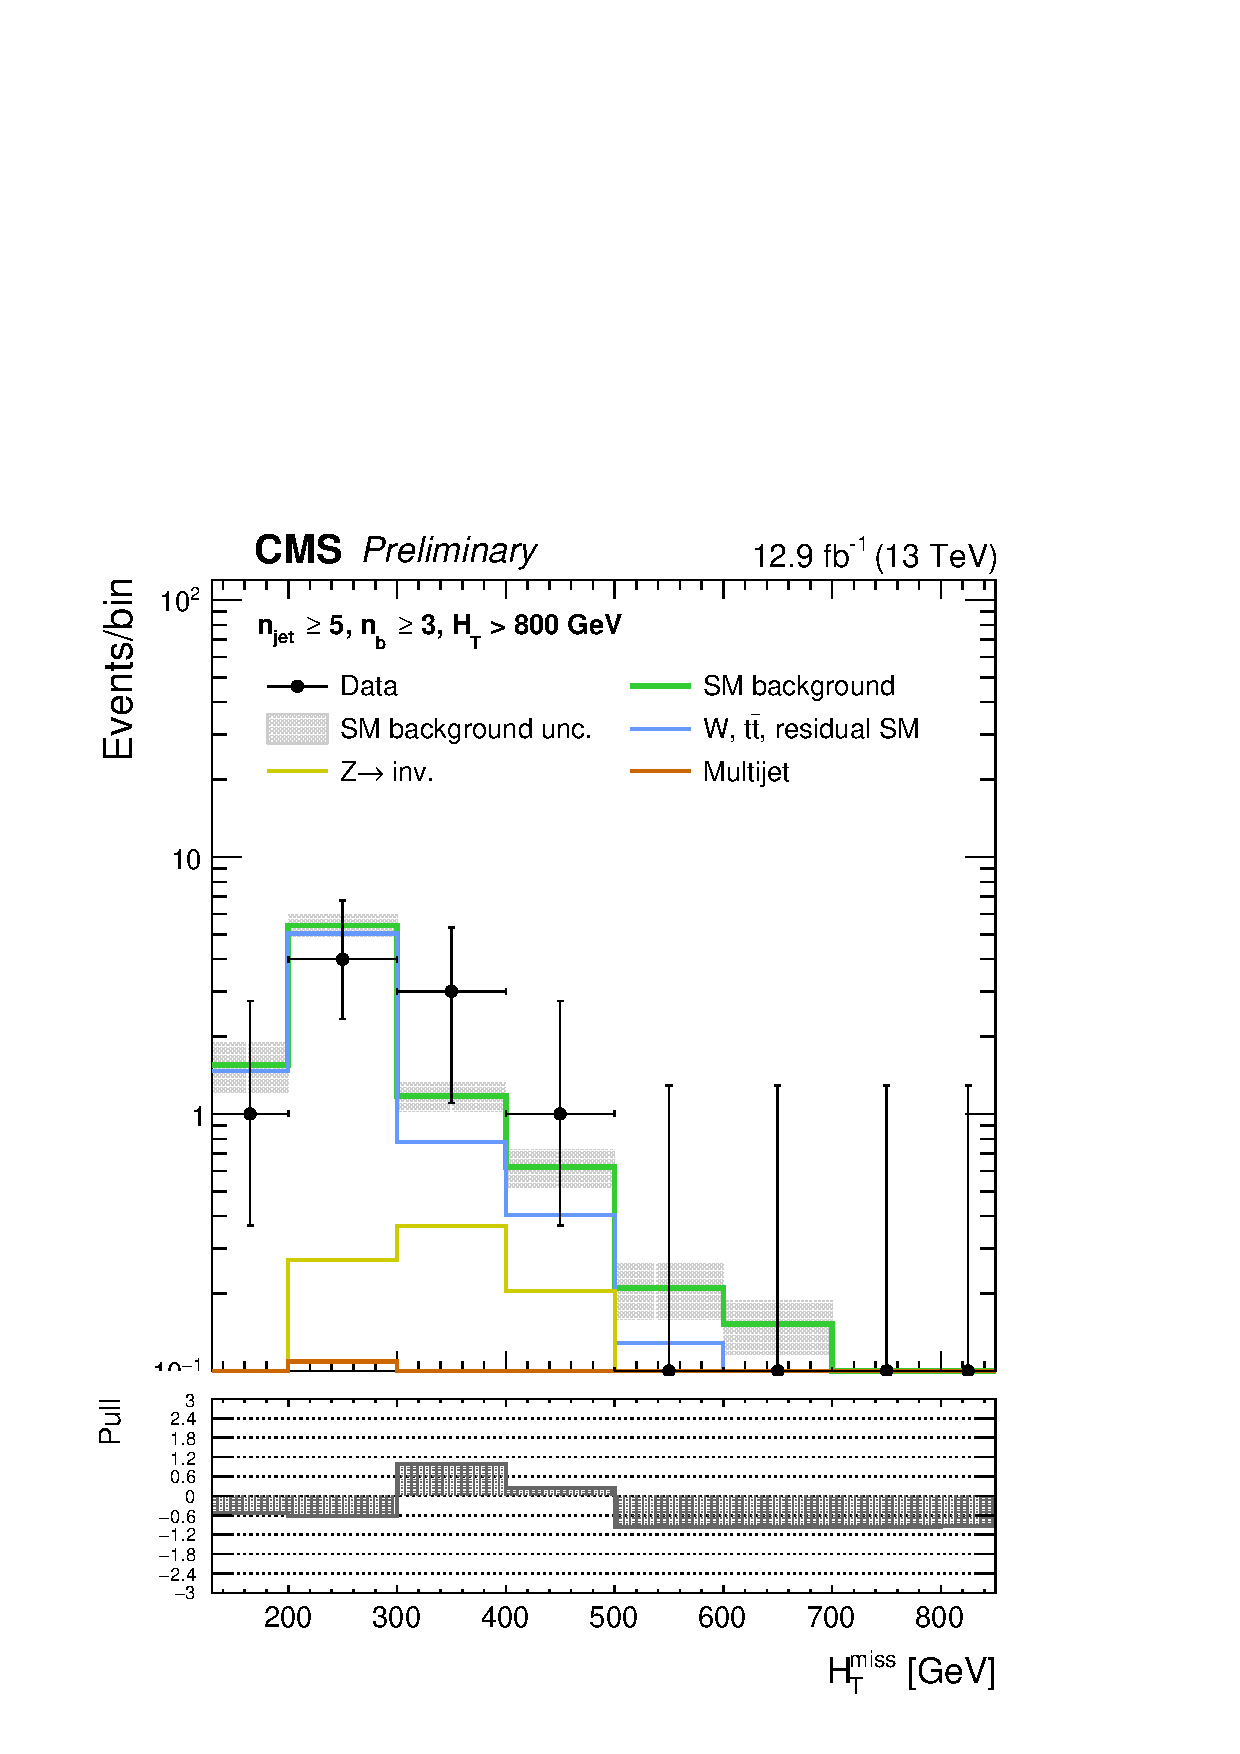
\includegraphics[width=0.49\textwidth]{Figures/statisticalResults/mhtShape_ge3b_ge5j_800_Inf_fit_b.pdf} 
  \end{center}
  \caption{Event yields observed in data (solid circles) and SM
    expectations from the CR-only fit with their associated
    uncertainties (green histogram with shaded band) as a function of
    \mht for events in the signal region that satisfy $\njet \geq
    5$, $\scalht > 800\GeV$, and (Left) $\nb = 0$ or (Right) $\nb \geq
    3$. The final bin is the overflow bin. The bottom panels indicate
    the significance of the deviations (pulls) observed in data with respect
    to the SM expectations, expressed in terms of the total
    uncertainty in the SM expectations. The pulls are indicative only
    and cannot be considered independently.  
    \label{fig:mht-templates} 
  }
\end{figure}

\clearpage
\section{Interpretation}

Given the agreement between prediction and results presented in Section ??, no evidence
for physics beyond the standard model is observed. The results are therefore used to constrain
the parameter space of simplified supersymmetric models (see Section ??). The simplified 
models considered are the gluino-mediated and direct production of
both bottom and top squark pairs. The \alphat~search is expected to be particularly to
such topologies due to the significant hadronic activity, bottom quarks, jet multiplicity
and \mht that may be present in the final state. Limits at 95\% confidence level (see Section~\ref{sec:limits}) 
are set on the production cross section of each model.

\subsection{Signal model contribution and systematic uncertainties}

The experimental efficiency times acceptance ($\epsilon \times A$) in both the signal and 
control regions is derived independantly for each signal model for each gluino or squark 
mass ($m_{\text{SUSY}}$) and neutrinalino mass ($m_{\tilde{\chi}^{0}}$). As for the 
background processes, the simulated events for the signal contribution are corrected for 
jet energy corrections, b tag scale factors, lepton scale factors, pile up modelling and trigger efficiencies.
In addition, a correction is made to account for differences observed in the initial 
state radiation modelling between data and simulation. Systematic uncertainties are included 
on each of these corrections, analagously to the background processes. The signal contribution
cannot be predicted using data and therefore the overall normalisation contains an uncertainty
from the luminosity measurement of 6.2\%. All systematics are summarised
in Table~\ref{tab:signal_systs} including typical magnitudes for direct bottom squark production.

\begin{table}[h!]
  \caption{
    Representative magnitudes of systematic uncertainties in the
    experimental acceptance for simplified models that assume the 
    pair production of bottom squarks and their decay to a b
    quark and a \chiz.}  
  \label{tab:signal_systs}
  \centering
  \footnotesize
  \begin{tabular}{ lccc }
    \hline
    Systematic source\T\B          & Correlated & Typical magnitude (\%) \\
    \hline
    Luminosity\T                   & Yes        & 6.2                    \\
    Monte Carlo statistics         & No         & 1--50                  \\
    Jet energy scale               & Yes        & 3--10                  \\
    b-tag efficiency scale factors & Yes        & 5--40                  \\
    Lepton scale factors           & Yes        & 1--5                   \\
    Pile-up                        & Yes        & 0--5                   \\
    Trigger efficiency             & Yes        & 0--4                   \\
    Initial state radiation        & Yes        & 1--20                  \\
%    Renormalisation/factorisation & Norm. + shape & No         & 10                     \\
    \hline
  \end{tabular}
\end{table}

\subsection{Procedure for deriving limits}
\label{sec:limits}
The results of the \alphat~search are interpreted by deriving upper limits on the signal strength
at 95\% confidence level for simplified models. This section describes the procedure for deriving
these upper limits. A more comprehensive treatment can be found in~\cite{asymp}.

In the following section the signal strength is considered as the parameter of interest (POI)
and all other parameters in the fit are termed the \emph{nuisance parameters} ($\boldsymbol{\theta}$). Considering
the likelihood defined in~\ref{eq:totalLikelihood}, the profile likelihood ratio can be defined as

\begin{equation}
\label{eq:profile}
\lambda(r) = \frac{\mathcal{L}(r,\hat{\boldsymbol{\theta}}(r))}{\mathcal{L}(\hat{r},\hat{\boldsymbol{\theta}})},
\end{equation}

where $\hat{\boldsymbol{\theta}}$ and $\hat{r}$ are the values of $\boldsymbol{\theta}$ and r that maximise $\mathcal{L}$
, maximum-likelihood (ML) estimators, while $\hat{\boldsymbol{\theta}}(r)$ is the value
of $\boldsymbol{\theta}$ that maximises $\mathcal{L}$ for the specified value of r. 

Given that $r < 0$ is unphysical the profile likelihood is modified as
\begin{equation}
\label{eq:profileNew}
\tilde{\lambda}(r) = 
\begin{cases}
\lambda(0)\quad r \le 0, \\ 
\lambda(r)\quad r > 0. \\ 
\end{cases}
\end{equation}

The test statistic used to derive the upper limit on r is then defined as

\begin{equation}
t_r = 
\begin{cases}
-2\,\text{ln}\,\tilde{\lambda(r)}\quad &\hat{r} \le r, \\ 
0 \quad &\hat{r} > r. \\ 
\end{cases}
\end{equation}

Considering Eq.~\ref{eq:profile}, $t_r$ will be zero at the ML value of r.
Increasing values of $t_r$ represent less compatibility of that value of r with
the observed data. The test statistic is set to zero for $\hat{r} > r$ as
values of r less than $\hat{r}$ are not part of the \emph{rejection region} for upper limits. 

The probability density function, $f(t_r|r)$, for $t_r$ may be built by 
generating pseudo datasets or approximated using the asymptotic formulae 
detailed in~\cite{asymp}. The \alphat~analysis uses the asymptotic
approximation for $f(t_r|r)$. The p-value, $p_r$, can then be defined as

\begin{equation}
p_r = \int_{t_{r,obs}}^{\infty}\, f(t_r|r)\, dt_r
\end{equation}

where ${t_{r,obs}}$ is the observed value of the test statistic. Finally,
the $\text{CLs}$ is defined as

\begin{equation}
\text{CLs}(r) = \frac{p_r}{1-p_0}.
\end{equation}

The upper limit on r is defined as the value of $r$ which corresponds to 
$\text{CLs}(r) = 0.05$ ($r_{95}$). Values of r greater than this are said to be excluded at 95\%
confidence level.

The expected limit on a given signal strength, $r_{95}^{exp}$, is defined by the median value of the distribution
of $r_{95}$ built from pseudo datasets generated with no signal contribution (r = 0). The variation in the 
expected limit may also be estimated by the relevant quantiles from this distributuon.
For the \alphat~analysis, the value and variations of $r_{95}^{exp}$ are approximated using 
the asymptotic formulae detailed in~\cite{asymp}.

\subsection{Upper limits}

In Figures~\ref{fig:limits-sms}, the upper limits at 95\% CL set on the production cross section are shown
in the ($m_{\text{SUSY}}$, $m_{\tilde{\chi}^{0}}$) plane for the models considered.
Also shown are the expected and observed contours of $r_{95} = 1$, the $\pm$ 1 and 2
$\sigma$ variations in the expected limit, and the observed limit under $\pm$ 1 $\sigma$ 
variations in the theoretical cross section uncertainty.

\begin{figure}[thp!]
  \begin{center}
    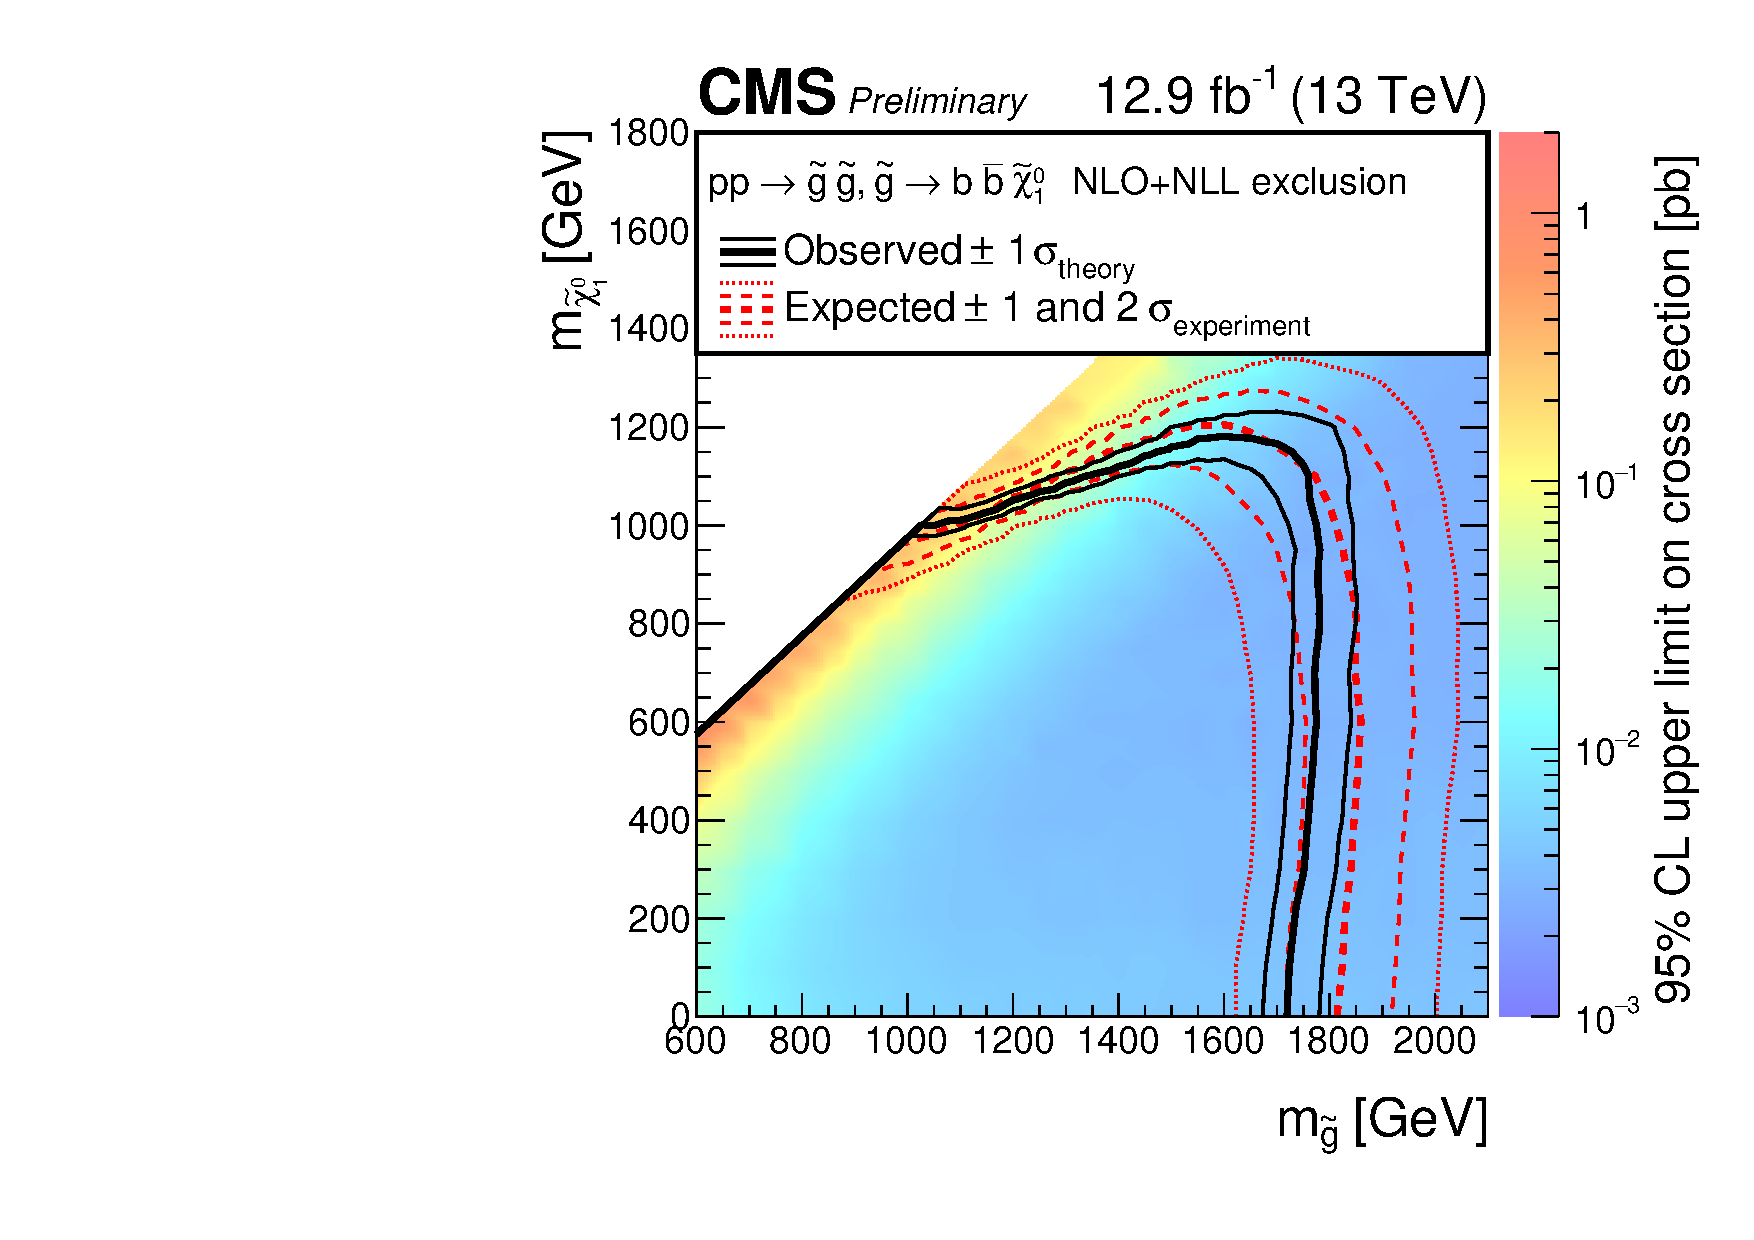
\includegraphics[width=0.45\textwidth]{./Figures/statisticalResults/SUS16T1bbbbXSEC.pdf} ~
    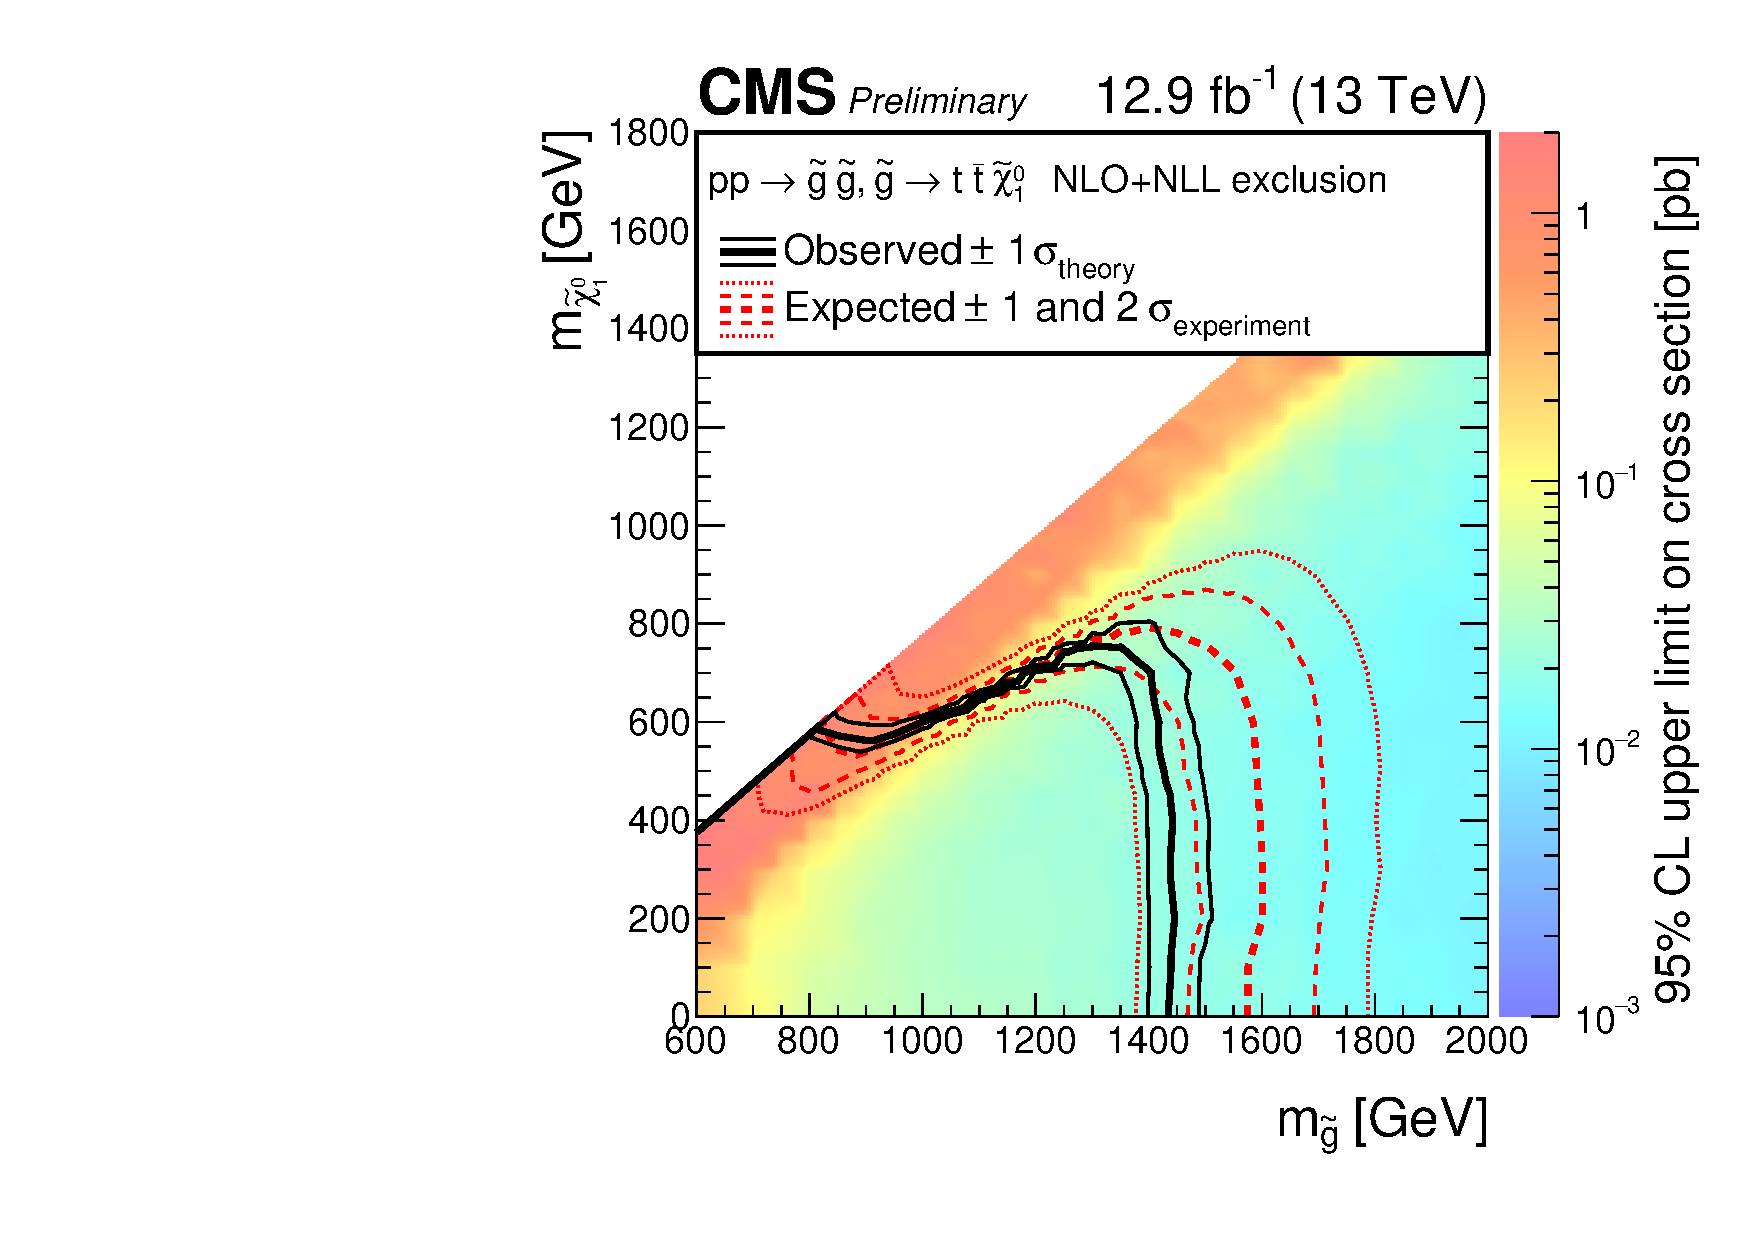
\includegraphics[width=0.45\textwidth]{./Figures/statisticalResults/SUS16T1ttttXSEC.pdf} \\
    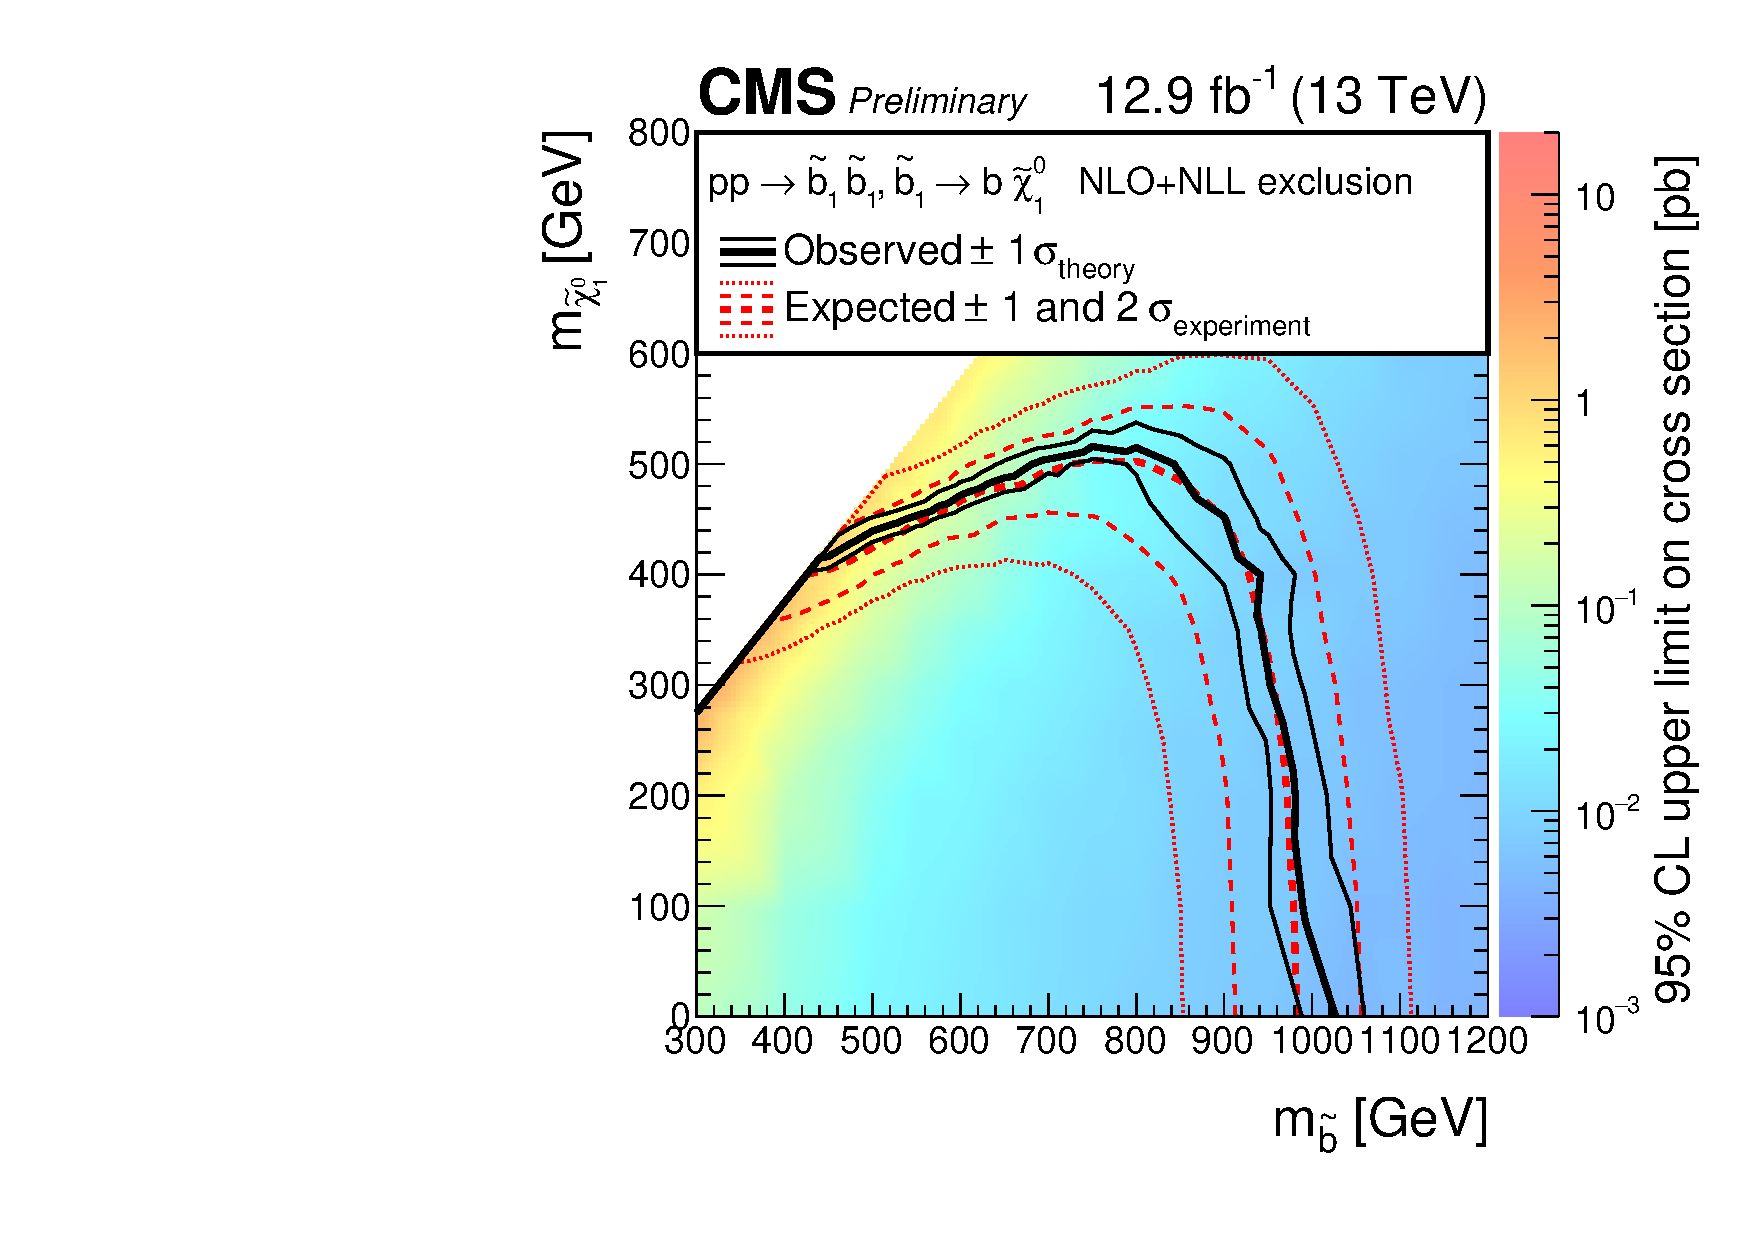
\includegraphics[width=0.45\textwidth]{./Figures/statisticalResults/SUS16T2bbXSEC.pdf} ~
    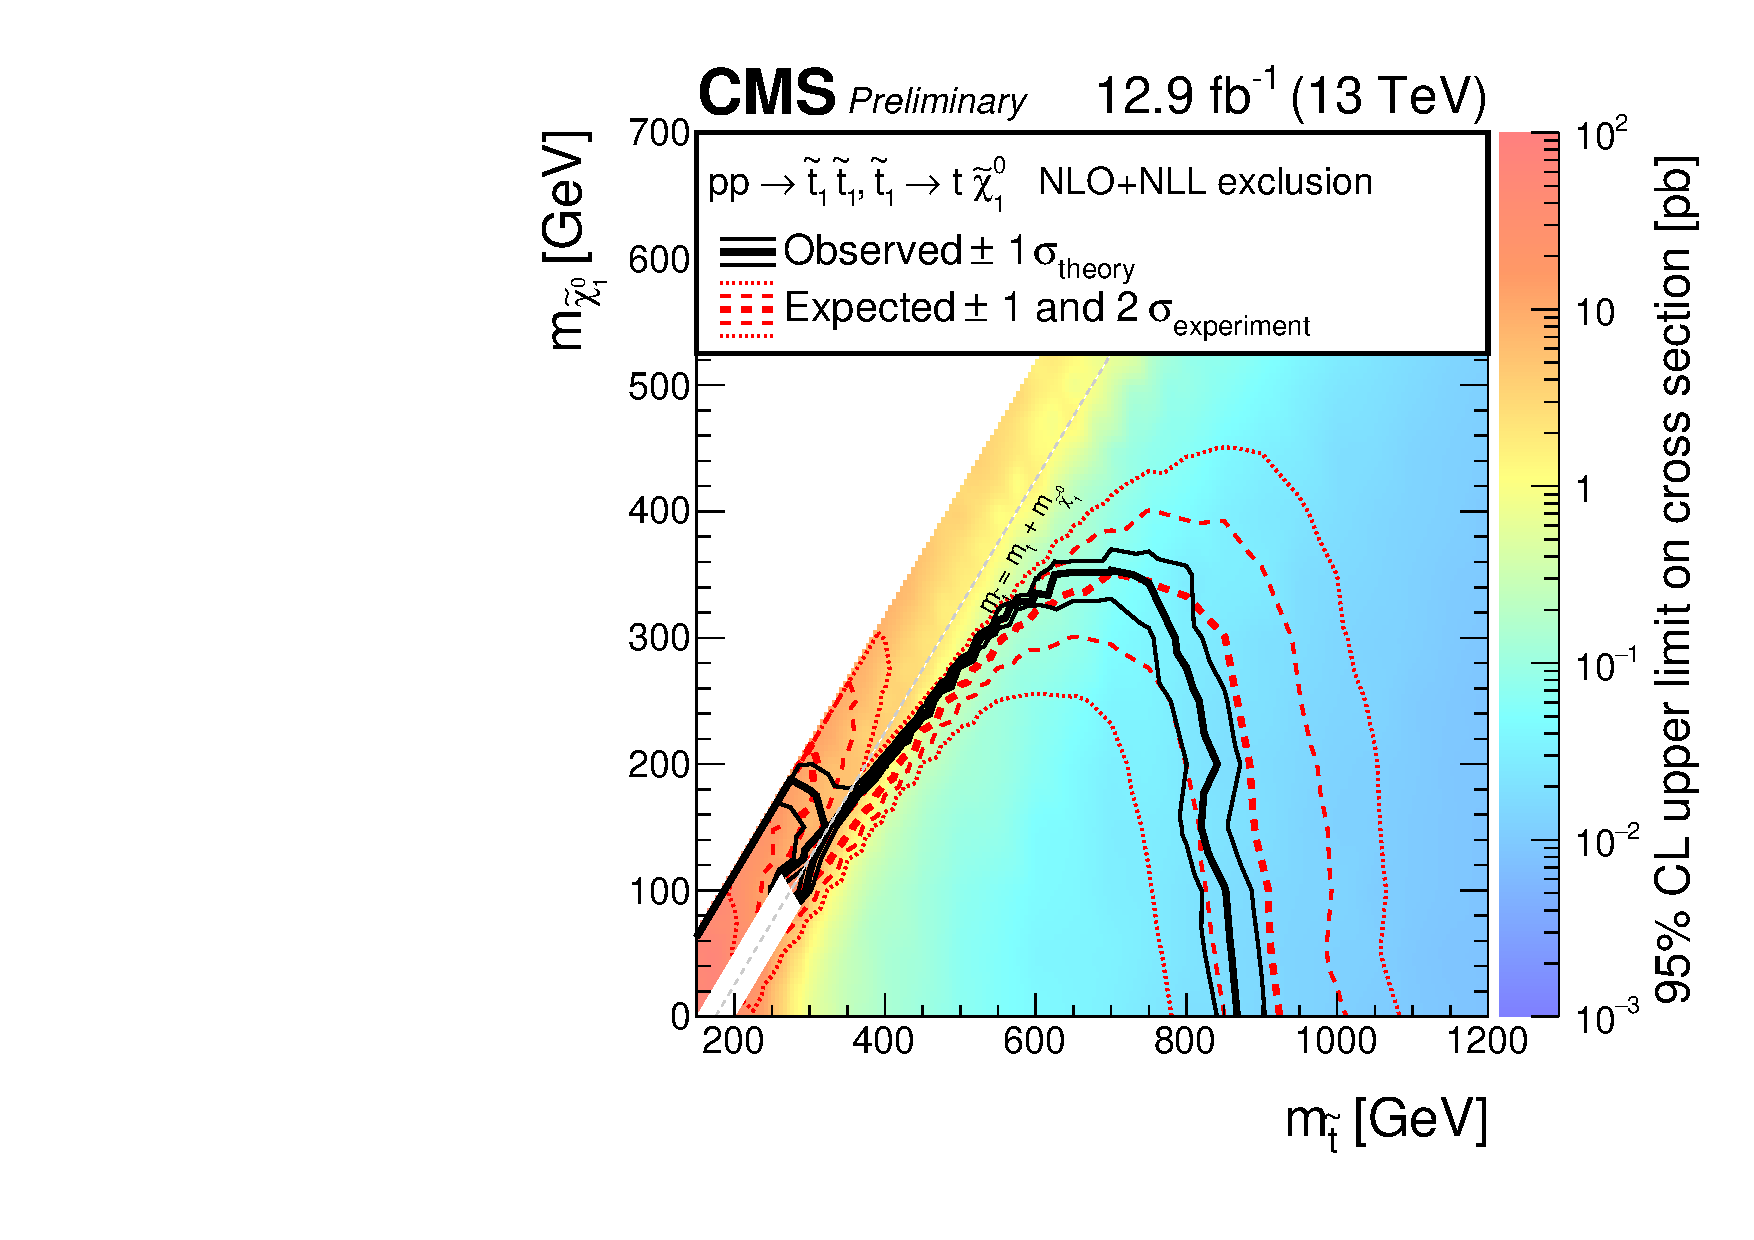
\includegraphics[width=0.45\textwidth]{./Figures/statisticalResults/SUS16T2ttXSEC.pdf} 
    \caption{Observed upper limit in cross section at 95\% confidence
      level (indicated by the colour scale) for simplified models that
      assume the (Top) gluino-mediated or (Bottom) direct production
      of (Left) bottom or (Right) top squark pairs, as a function of
      the gluino or squark mass and the $\chiz_{1}$ 
      mass. The black solid thick (thin) line indicates the observed
      mass exclusion regions assuming the nominal (${\pm}1 \sigma$
      theory uncertainty) production cross section. The red dashed
      thick (thin) line indicates the median (${\pm}1 \sigma$
      experimental uncertainty) expected mass exclusion
      regions. 
      \label{fig:limits-sms} }
  \end{center}
\end{figure}
